% Options for packages loaded elsewhere
\PassOptionsToPackage{unicode}{hyperref}
\PassOptionsToPackage{hyphens}{url}
\PassOptionsToPackage{dvipsnames,svgnames,x11names}{xcolor}
%
\documentclass[
]{article}
\usepackage{amsmath,amssymb}
\usepackage{lmodern}
\usepackage{setspace}
\usepackage{iftex}
\ifPDFTeX
  \usepackage[T1]{fontenc}
  \usepackage[utf8]{inputenc}
  \usepackage{textcomp} % provide euro and other symbols
\else % if luatex or xetex
  \usepackage{unicode-math}
  \defaultfontfeatures{Scale=MatchLowercase}
  \defaultfontfeatures[\rmfamily]{Ligatures=TeX,Scale=1}
\fi
% Use upquote if available, for straight quotes in verbatim environments
\IfFileExists{upquote.sty}{\usepackage{upquote}}{}
\IfFileExists{microtype.sty}{% use microtype if available
  \usepackage[]{microtype}
  \UseMicrotypeSet[protrusion]{basicmath} % disable protrusion for tt fonts
}{}
\makeatletter
\@ifundefined{KOMAClassName}{% if non-KOMA class
  \IfFileExists{parskip.sty}{%
    \usepackage{parskip}
  }{% else
    \setlength{\parindent}{0pt}
    \setlength{\parskip}{6pt plus 2pt minus 1pt}}
}{% if KOMA class
  \KOMAoptions{parskip=half}}
\makeatother
\usepackage{xcolor}
\IfFileExists{xurl.sty}{\usepackage{xurl}}{} % add URL line breaks if available
\IfFileExists{bookmark.sty}{\usepackage{bookmark}}{\usepackage{hyperref}}
\hypersetup{
  pdftitle={A general model for the evolution of nuptial gift-giving: Supporting Information},
  colorlinks=true,
  linkcolor={blue},
  filecolor={Maroon},
  citecolor={Blue},
  urlcolor={Blue},
  pdfcreator={LaTeX via pandoc}}
\urlstyle{same} % disable monospaced font for URLs
\usepackage[margin=1in]{geometry}
\usepackage{color}
\usepackage{fancyvrb}
\newcommand{\VerbBar}{|}
\newcommand{\VERB}{\Verb[commandchars=\\\{\}]}
\DefineVerbatimEnvironment{Highlighting}{Verbatim}{commandchars=\\\{\}}
% Add ',fontsize=\small' for more characters per line
\usepackage{framed}
\definecolor{shadecolor}{RGB}{248,248,248}
\newenvironment{Shaded}{\begin{snugshade}}{\end{snugshade}}
\newcommand{\AlertTok}[1]{\textcolor[rgb]{0.94,0.16,0.16}{#1}}
\newcommand{\AnnotationTok}[1]{\textcolor[rgb]{0.56,0.35,0.01}{\textbf{\textit{#1}}}}
\newcommand{\AttributeTok}[1]{\textcolor[rgb]{0.77,0.63,0.00}{#1}}
\newcommand{\BaseNTok}[1]{\textcolor[rgb]{0.00,0.00,0.81}{#1}}
\newcommand{\BuiltInTok}[1]{#1}
\newcommand{\CharTok}[1]{\textcolor[rgb]{0.31,0.60,0.02}{#1}}
\newcommand{\CommentTok}[1]{\textcolor[rgb]{0.56,0.35,0.01}{\textit{#1}}}
\newcommand{\CommentVarTok}[1]{\textcolor[rgb]{0.56,0.35,0.01}{\textbf{\textit{#1}}}}
\newcommand{\ConstantTok}[1]{\textcolor[rgb]{0.00,0.00,0.00}{#1}}
\newcommand{\ControlFlowTok}[1]{\textcolor[rgb]{0.13,0.29,0.53}{\textbf{#1}}}
\newcommand{\DataTypeTok}[1]{\textcolor[rgb]{0.13,0.29,0.53}{#1}}
\newcommand{\DecValTok}[1]{\textcolor[rgb]{0.00,0.00,0.81}{#1}}
\newcommand{\DocumentationTok}[1]{\textcolor[rgb]{0.56,0.35,0.01}{\textbf{\textit{#1}}}}
\newcommand{\ErrorTok}[1]{\textcolor[rgb]{0.64,0.00,0.00}{\textbf{#1}}}
\newcommand{\ExtensionTok}[1]{#1}
\newcommand{\FloatTok}[1]{\textcolor[rgb]{0.00,0.00,0.81}{#1}}
\newcommand{\FunctionTok}[1]{\textcolor[rgb]{0.00,0.00,0.00}{#1}}
\newcommand{\ImportTok}[1]{#1}
\newcommand{\InformationTok}[1]{\textcolor[rgb]{0.56,0.35,0.01}{\textbf{\textit{#1}}}}
\newcommand{\KeywordTok}[1]{\textcolor[rgb]{0.13,0.29,0.53}{\textbf{#1}}}
\newcommand{\NormalTok}[1]{#1}
\newcommand{\OperatorTok}[1]{\textcolor[rgb]{0.81,0.36,0.00}{\textbf{#1}}}
\newcommand{\OtherTok}[1]{\textcolor[rgb]{0.56,0.35,0.01}{#1}}
\newcommand{\PreprocessorTok}[1]{\textcolor[rgb]{0.56,0.35,0.01}{\textit{#1}}}
\newcommand{\RegionMarkerTok}[1]{#1}
\newcommand{\SpecialCharTok}[1]{\textcolor[rgb]{0.00,0.00,0.00}{#1}}
\newcommand{\SpecialStringTok}[1]{\textcolor[rgb]{0.31,0.60,0.02}{#1}}
\newcommand{\StringTok}[1]{\textcolor[rgb]{0.31,0.60,0.02}{#1}}
\newcommand{\VariableTok}[1]{\textcolor[rgb]{0.00,0.00,0.00}{#1}}
\newcommand{\VerbatimStringTok}[1]{\textcolor[rgb]{0.31,0.60,0.02}{#1}}
\newcommand{\WarningTok}[1]{\textcolor[rgb]{0.56,0.35,0.01}{\textbf{\textit{#1}}}}
\usepackage{longtable,booktabs,array}
\usepackage{calc} % for calculating minipage widths
% Correct order of tables after \paragraph or \subparagraph
\usepackage{etoolbox}
\makeatletter
\patchcmd\longtable{\par}{\if@noskipsec\mbox{}\fi\par}{}{}
\makeatother
% Allow footnotes in longtable head/foot
\IfFileExists{footnotehyper.sty}{\usepackage{footnotehyper}}{\usepackage{footnote}}
\makesavenoteenv{longtable}
\usepackage{graphicx}
\makeatletter
\def\maxwidth{\ifdim\Gin@nat@width>\linewidth\linewidth\else\Gin@nat@width\fi}
\def\maxheight{\ifdim\Gin@nat@height>\textheight\textheight\else\Gin@nat@height\fi}
\makeatother
% Scale images if necessary, so that they will not overflow the page
% margins by default, and it is still possible to overwrite the defaults
% using explicit options in \includegraphics[width, height, ...]{}
\setkeys{Gin}{width=\maxwidth,height=\maxheight,keepaspectratio}
% Set default figure placement to htbp
\makeatletter
\def\fps@figure{htbp}
\makeatother
\setlength{\emergencystretch}{3em} % prevent overfull lines
\providecommand{\tightlist}{%
  \setlength{\itemsep}{0pt}\setlength{\parskip}{0pt}}
\setcounter{secnumdepth}{-\maxdimen} % remove section numbering
\newlength{\cslhangindent}
\setlength{\cslhangindent}{1.5em}
\newlength{\csllabelwidth}
\setlength{\csllabelwidth}{3em}
\newlength{\cslentryspacingunit} % times entry-spacing
\setlength{\cslentryspacingunit}{\parskip}
\newenvironment{CSLReferences}[2] % #1 hanging-ident, #2 entry spacing
 {% don't indent paragraphs
  \setlength{\parindent}{0pt}
  % turn on hanging indent if param 1 is 1
  \ifodd #1
  \let\oldpar\par
  \def\par{\hangindent=\cslhangindent\oldpar}
  \fi
  % set entry spacing
  \setlength{\parskip}{#2\cslentryspacingunit}
 }%
 {}
\usepackage{calc}
\newcommand{\CSLBlock}[1]{#1\hfill\break}
\newcommand{\CSLLeftMargin}[1]{\parbox[t]{\csllabelwidth}{#1}}
\newcommand{\CSLRightInline}[1]{\parbox[t]{\linewidth - \csllabelwidth}{#1}\break}
\newcommand{\CSLIndent}[1]{\hspace{\cslhangindent}#1}
\usepackage{amsmath}
\usepackage{natbib}
\usepackage{lineno}
\usepackage{caption}
\usepackage[utf8]{inputenc}
\bibliographystyle{amnatnat}
\ifLuaTeX
  \usepackage{selnolig}  % disable illegal ligatures
\fi

\title{A general model for the evolution of nuptial gift-giving:
Supporting Information}
\author{Anders P. Charmouh\(^{1,4, 5}\), Trine Bilde\(^{2}\), Greta
Bocedi\(^{1}\), A. Bradley Duthie\(^{3}\)}
\date{{[}1{]} School of Biological Sciences, University of Aberdeen, UK.
{[}2{]} Department of Biology, Aarhus University, Denmark. {[}3{]}
Biological and Environmental Sciences, University of Stirling, UK.
{[}4{]} Bioinformatics Research Centre Aarhus University, University
City 81, building 1872, 3rd floor, DK-8000 Aarhus C, Denmark {[}5{]}
Email: \href{mailto:apc@birc.au.dk}{\nolinkurl{apc@birc.au.dk}}}

\begin{document}
\maketitle

\setstretch{1}
\hypertarget{table-of-contents}{%
\section{Table of Contents}\label{table-of-contents}}

\begin{longtable}[]{@{}ll@{}}
\toprule
Information & Page \\
\midrule
\endhead
S1: Description of the individual-based simulation model & 2 \\
S2: Sensitivity analysis of mortality parameters in IBM & 4 \\
S3: Alternative derivation of male fitness threshold & 14 \\
S4: Operational sex ratio & 16 \\
S5: Estimation of key model parameter using experimental data & 17 \\
S6: Separate evolution of male search and female choice & 18 \\
References & 19 \\
\bottomrule
\end{longtable}

\clearpage

\hypertarget{s1-description-of-the-individual-based-simulation-model}{%
\subsection{S1: Description of the individual-based simulation
model}\label{s1-description-of-the-individual-based-simulation-model}}

Here we describe the details of initialisation, time-in (mating),
time-out (reproduction and nuptial gift search), and mortality. We then
summarise the simulations run and data collected.

\emph{Initialisation}

Before the first time step, a population of \(N = 1000\) individuals is
initialised. Individuals are assigned unique IDs, and each is assigned
to be female with a probability of \(0.5\), else male. Each individual
\(i\) is initialised with a starting value of female offspring
processing time (\(T^{i}_{\mathrm{f}}\)), rejection probability of
gift-less males (\(\rho^{i}\)), and male search time
(\(T^{i}_{\mathrm{m}}\)). For all simulations, initialised values are
set to \(T^{i}_{\mathrm{f}} = 2\), \(\rho^{i} = 0\), and
\(T^{i}_{\mathrm{m}} = 0\). All individuals are initalised outside of
the mating pool in the first time step \(t = 1\). The first time step
then proceeds with females immediately entering the mating pool and
males either entering the mating pool or searching for nuptial gifts.

\emph{Time-in}

At the start of each time step, females and males in the mating pool
remain in it. Females will enter the mating pool after processing
offspring, and males will enter it after searching for nuptial gifts
(see `Time-out' below). Up to \(\Psi = N\psi\) interactions between
individuals can occur in a single time step, where \(N\) is population
size and \(\psi\) is a scaling parameter. In each time step, \(\Psi\)
pairs of individuals are selected at random to interact. For each
interaction, two different individuals are randomly selected from the
population with equal probability. If the selected individuals are of
different sexes, and both are in the mating pool, then a mating
encounter occurs. If the male does not have a nuptial gift, then the
female will reject him with a probability of \(\rho^{i}\); if rejection
occurs, then both individuals stay in the mating pool. If rejection does
not occur, or the male has a nuptial gift in the mating encounter, then
the individuals mate. Females leave the mating pool and enter time-out
to process offspring, and males leave and enter time-out to potentially
search for new nuptial gifts (note that females and males might re-enter
the mating pool immediately within the same time step given sufficiently
low search time; see Time-out below).

\emph{Time-out}

During time-out, offspring production and time outside of the mating
pool are realised for each female by sampling from a Poisson
distribution. A focal female \(i\) will produce \(Poisson(\lambda)\)
offspring if no nuptial gift was provided or
\(Poisson(\lambda + \gamma)\) if a gift was provided. Females remain
outside of the mating pool to process offspring for
\(Poisson(T^{i}_{\mathrm{f}})\) time steps. Offspring are added to the
population immediately, with \(\rho^{i}\) and \(T^{i}_{\mathrm{m}}\)
values that are the average of each parent plus some normally
distributed error \(\epsilon_{R}\) and \(\epsilon_{T_{\mathrm{m}}}\).
For example,

\[T^{\mathrm{offspring}}_{\mathrm{m}} \sim \frac{T^{\mathrm{mother}}_{\mathrm{m}}  + T^{\mathrm{father}}_{\mathrm{m}}}{2} + N\left(0, \epsilon_{T_{\mathrm{m}}} \right).\]

The variation generated by \(\epsilon\) values simulates mutation upon
which selection for traits can act. In all simulations, \(\epsilon = 0\)
if a trait is fixed and \(\epsilon = 0.01\) if the trait evolves.
Offspring sex is randomly assigned with equal probability as female or
male. Female offspring are immediately placed in the mating pool, and
male offspring are out of the mating pool to potentially search for
nuptial gifts. After a female has spent \(T^{i}_{\mathrm{f}}\) time
steps outside the mating pool, she will re-enter it.

A focal male \(i\) outside the mating pool will enter it if he has
searched for a fixed number of \(T^{i}_{\mathrm{m}}\) time steps, which
is also sampled randomly from a Poisson distribution,
\(Poisson(T^{i}_{\mathrm{m}})\). If \(T^{i}_{\mathrm{m}} = 0\), then the
male immediately returns to the mating pool (in the same time step). If
\(T^{i}_{\mathrm{m}} > 0\), then the male must wait outside the mating
pool for \(Poisson(T^{i}_{\mathrm{m}})\) time steps, but will enter the
mating pool with a nuptial gift with a probability,

\[P(G^{i}) = 1 - e^{-\frac{1}{\alpha}T^{i}_{\mathrm{m}}}.\]

Males must always spend \(T^{i}_{\mathrm{m}}\) time steps outside of the
mating pool regardless of whether or not they are successful in
obtaining a nuptial gift.

\emph{Mortality}

At the end of each time step, mortality occurs first with a fixed
probability for all adults in the population, then with a probability
caused by carrying capacity \(K\) applied to all individuals (adults and
offspring). Mortality occurs in each time step with a fixed probability
of \(\mu\) regardless of the sex of the individual or its position in or
out of the mating pool. If after this fixed mortality is applied, the
total population size \(N > K\), then individuals are removed at random
with equal probability until \(N = K\). Following adult mortality, a new
time step begins with newly added offspring becoming adults.

\emph{Simulations}

We ran simulations in which male search time and female choosiness
evolved from an ancestral state of no searching and no choosiness. In
all simulations, \(N\) was initialised at 1000 and \(K = 1000\).
Simulations ran for \(t_{max} = 40000\) time steps. We set
\(T_{\mathrm{f}} = 2\), \(\psi = 3\), and \(\lambda = 1\) for all
simulations, and we simulated across a range of
\(\alpha = \{0.1, 0.2, ..., 1.9, 2.0\}\) and
\(\gamma = \{0, 0.1, ..., 1.9, 2.0\}\) parameter values for 3200
replicates. Summary statistics for mean trait values, population size,
sex ratios, proportion of females and males in and out of the mating
pool, and mean number of encounters per female and male within the
mating pool were all calculated in the last time step. The C code used
for simulating these IBMs also allows for the reporting of statistics in
each time step. Additionally, it can simulate explicit space and
individual movement through the landscape. A neutral evolving trait was
also modelled to ensure that the code functioned as intended, and
processes were compartmentalised into individual functions to facilitate
code testing. All code is publicly available on GitHub
(\url{https://github.com/bradduthie/nuptial_gift_evolution}).

A set of simulations with a value of \(\gamma\) calculated from
empirical data was also conducted (100 replicates). Here, \(\gamma\) was
parameterised using data on egg production as a function of eating
nuptial gifts (see below). Additional simulation sets with lower and
upper bounds of the estimated \(\gamma\) were subsequently run. In the
simulation sets with experimentally derived parameter values, all other
parameters were identical to previous simulation batches.

We can produce an estimate of the fitness increment obtained by females
when receiving a gift (\(\hat{\gamma}\)) by using data on female
\emph{P. mirabilis} egg production and hatching success under different
feeding regimes from (\protect\hyperlink{ref-Tuni2013a}{Tuni \emph{et
al.}, 2013}). Tuni \emph{et al.}
(\protect\hyperlink{ref-Tuni2013a}{2013}) found differences in egg
production and hatching success in female \emph{P. mirabilis} under
different feeding regimes. Assuming these differences in feeding regimes
correspond to eating versus not eating nuptial gifts, the mean number of
offspring produced by a female who eats nuptial gifts can be calculated
(Table 1).

\clearpage

\hypertarget{s2-sensitivity-analysis-of-parameters-in-ibm}{%
\subsection{S2: Sensitivity analysis of parameters in
IBM}\label{s2-sensitivity-analysis-of-parameters-in-ibm}}

We investigated the sensitivity of our results to individual mortality
during time-in (\(\mu_{\mathrm{in}}\)) and time-out
(\(\mu_{\mathrm{out}}\)), female processing time (\(T_{\mathrm{f}}\)),
potential for interactions between conspecifics (\(\psi\)), and
initialised male search time (\(T_{\mathrm{m}}\)). Across all of these
simulations, there were challenges with statistical power. Evidence for
the evolution of male search (blue points in figures) and female
choosiness (red points in figures) was determined by the lower 95\%
bootstrapped confidence interval of \(T_{\mathrm{m}}\) and
\(T_{\mathrm{f}}\) values being greater than zero, respectively. This
required a lot of replicate simulations in the main text (Figure 3),
especially for values just above predicted thresholds and for female
choosiness. Computation time was a limiting factor, even using a
compiled language (C) and with access to a computing cluster. Absence of
points above threshold values are not necessarily evidence that
evolution of male search or female choosiness is not predicted to evolve
in these regions of parameter space, but it does indicate that evolution
of these traits is not necessarily assured given the stochasticity
inherent to the IBM. Additional simulations can be conducted using the C
code in the `src' folder of the GitHub repository
(\url{https://github.com/bradduthie/nuptial_gift_evolution}). Below, we
explain the parameter values used in the sensitivity analysis in more
detail.

\emph{Mortality}

We conducted a sensitivity analysis of the effect of the mortality
parameters \(\mu_{\mathrm{in}}\) and \(\mu_{\mathrm{out}}\) (the
probability of mortality in time-in and time-out, respectively, which we
assumed to be equal for all individuals) on the evolution of male search
and female choice using the IBM (See S1). The results revealed no
correlation between the value of the mortality parameters and the
evolution of male search or female choice (Fig. S2.1).

\emph{Female processing time}

We also conducted a sensitivity analysis of female processing time
\(T_{\mathrm{f}}\). To do this, we ran simulations at default values,
but with \(T_{\mathrm{f}} = 0.4\) (Figure S4.2) and
\(T_{\mathrm{f}} = 10.0\) (Figures S4.3).

\emph{Interactions between conspecifics}

We conducted a sensitivity analysis on the encounter rate between
conspecifics (\(R\)) by varying the value of \(\psi\) (see S1). Under
default simulations, \(\psi = 3\). We also ran simulations in which
\(\psi = 1\) (Figure S4.4), \(\psi = 2\) (Figure S4.5), \(\psi = 4\)
(Figure S4.6), and \(\psi = 6\) (Figure S4.7), with all other parameters
being set to default values.

\emph{Initialised male search time}

Lastly, we conducted a sensitivity analysis on initialised male search
time (\(T_{\mathrm{m}}\)). To do this, we ran simulations at default
values, but initialised all males at \(T_{\mathrm{m}} = 0.5\) (Figure
S4.8) or \(T_{\mathrm{m}} = 2.5\) (S4.9). Note that under these
initialisation conditions, it no longer makes sense to test whether or
not \(T_{\mathrm{m}}\) evolves to positive values, so we do not show
predicted male search thresholds and focus only on female choosiness.
Interestingly, while predictions given initialised
\(T_{\mathrm{m}} = 0.5\) are quite close for female choosiness
thresholds, female choosiness does not appear to evolve given
\(T_{\mathrm{m}} = 2.5\). This might be due to low selection pressure to
reject males without gifts due to their low frequency. In other words,
while females would benefit from a strategy of rejecting gift-less
males, a lack of realised encounters with gift-less males preclude the
evolution of sustained selection for choosiness.

\clearpage

\captionsetup{labelformat=empty}

\begin{figure}
\centering
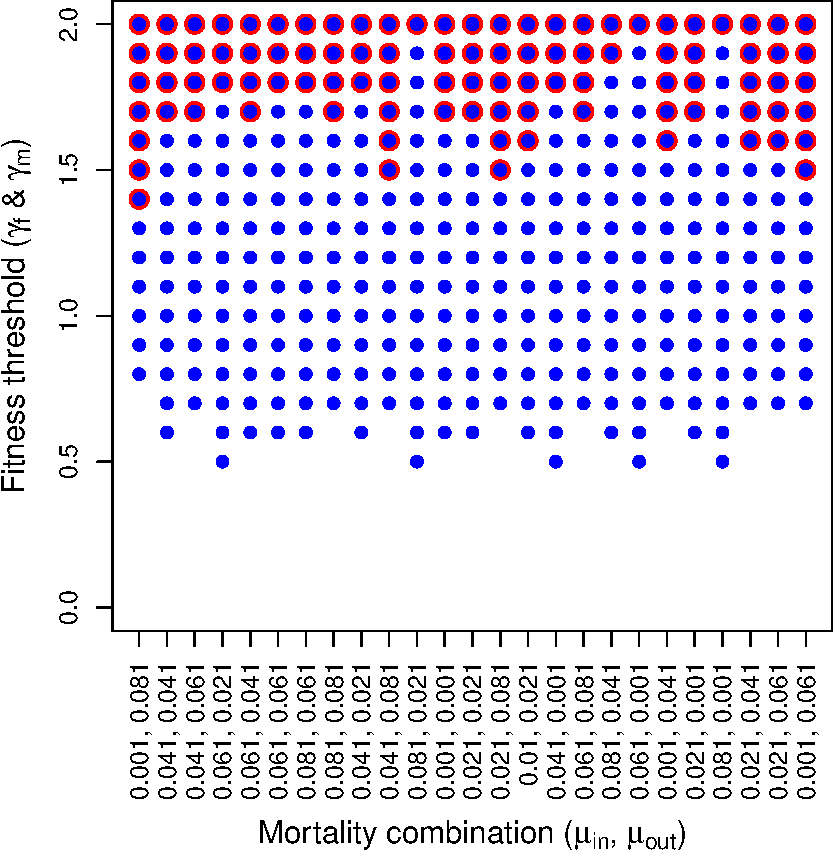
\includegraphics{SI_files/figure-latex/unnamed-chunk-2-1.pdf}
\caption{Figure S2.1: Evolution of both male search (blue) and female
choice (red) under different combinations of the mortality rates
\(\mu_{\mathrm{in}}\) and \(\mu_{\mathrm{out}}\) (mortality in time-in
and out, respectively). The y-axis is the threshold fitness that leads
to evolution of male search (blue) or female choice (red). The results
show noise, but no correlation between the value of the mortality
parameters and the propensity for male search and/or female choice to
evolve. For each of the \(25 \times 20\) combinations of
\(\mu_{\mathrm{in}}\) and \(\mu_{\mathrm{out}}\), 1600 replicate
simulations were run.}
\end{figure}

\captionsetup{labelformat=default}

\clearpage

\captionsetup{labelformat=empty}

\begin{figure}
\centering
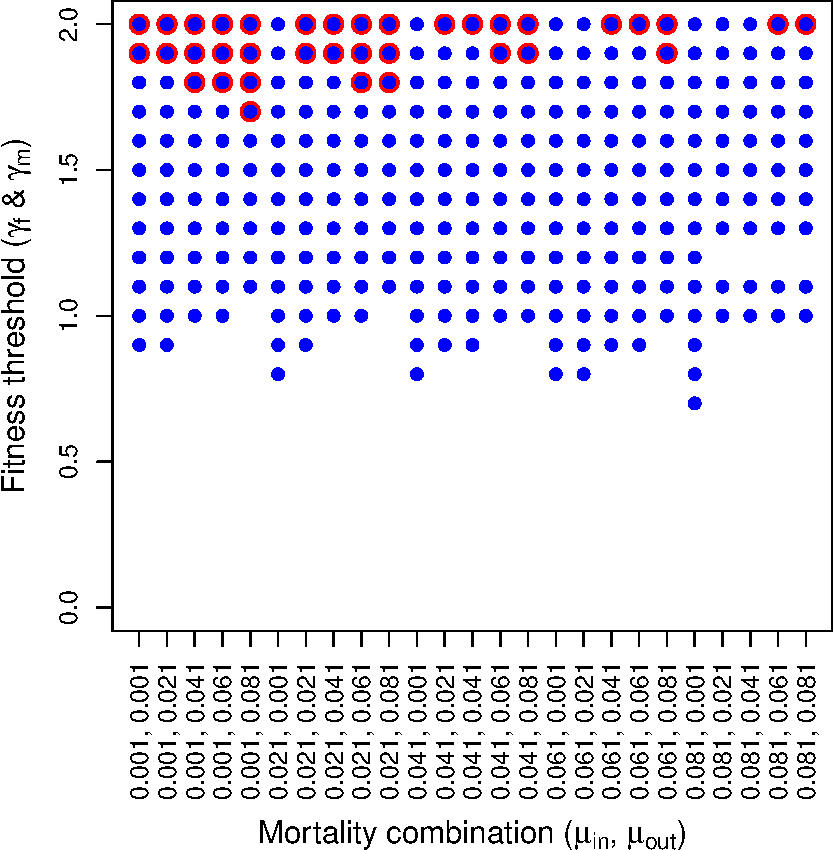
\includegraphics{SI_files/figure-latex/unnamed-chunk-3-1.pdf}
\caption{Figure S2.2 (\(T_{\mathrm{f}} = 0.5\)): The coevolution of male
search and female choosiness as a function of nuptial gift search time
(\(\alpha\)). Points show where the lower 95\% confidence interval of
female choosiness (red) and male search (blue) exceeds zero, indicating
evolution of choosiness or nuptial gift search. Each point includes data
from approximately 1600 replicate simulations with identical starting
conditions (some parameter combinations have fewer replicates). Red and
blue lines show thresholds above which the mathematical model predicts
that females should be choosy and males should search, respectively. Up
to 3000 interactions occur between individuals in each time step
(\(\psi = 3\)), potentially resulting in a mating interaction. The
number of individuals in the population remained at or near carrying
capacity of \(K = 1000\). Expected female processing time was set to
\(T_{\mathrm{f}}=0.5\) time steps, and \(\gamma\) and \(\alpha\) values
in the range {[}0.5, 1.5{]} and {[}0.1, 2.1{]}, respectively, were
used.}
\end{figure}

\captionsetup{labelformat=default}

\clearpage

\captionsetup{labelformat=empty}

\begin{figure}
\centering
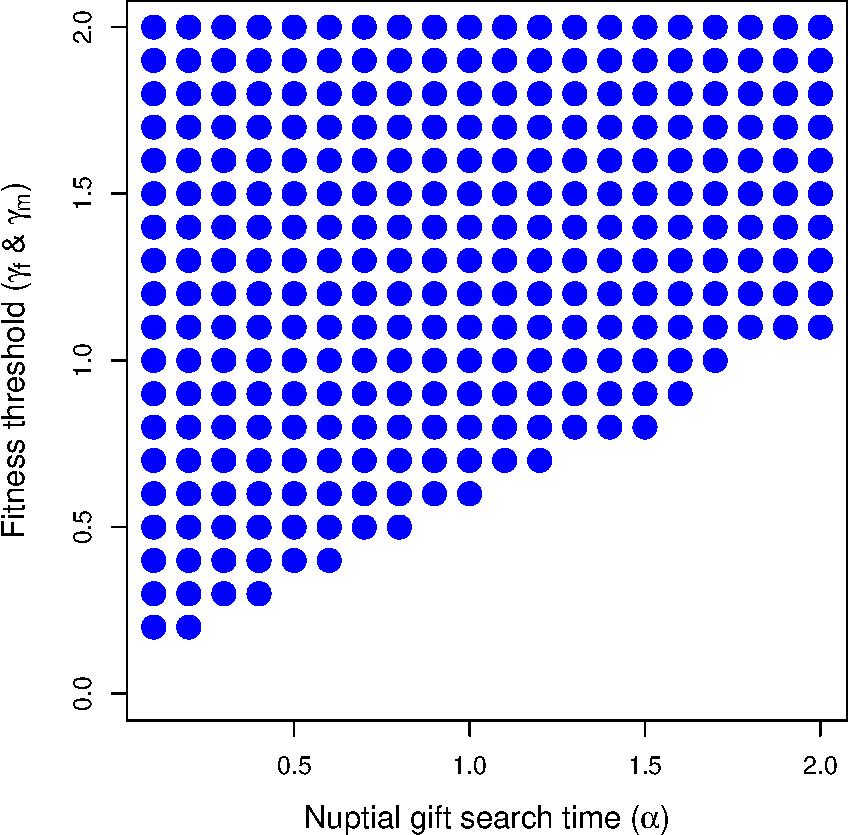
\includegraphics{SI_files/figure-latex/unnamed-chunk-4-1.pdf}
\caption{Figure S2.3 (\(T_{\mathrm{f}} = 10.0\)): The coevolution of
male search and female choosiness as a function of nuptial gift search
time (\(\alpha\)). Points show where the lower 95\% confidence interval
of female choosiness (red) and male search (blue) exceeds zero,
indicating evolution of choosiness or nuptial gift search. Each point
includes data from approximately 1600 replicate simulations with
identical starting conditions (some parameter combinations include fewer
replicates). Red and blue lines show thresholds above which the
mathematical model predicts that females should be choosy and males
should search, respectively. Up to 3000 interactions occur between
individuals in each time step (\(\psi = 3\)), potentially resulting in a
mating interaction. The number of individuals in the population remained
at or near carrying capacity of \(K = 1000\). Expected female processing
time was set to \(T_{\mathrm{f}}=10.0\) time steps, and \(\gamma\) and
\(\alpha\) values in the range {[}0.5, 1.5{]} and {[}0.1, 2.1{]},
respectively, were used.}
\end{figure}

\captionsetup{labelformat=default}

\clearpage

\captionsetup{labelformat=empty}

\begin{figure}
\centering
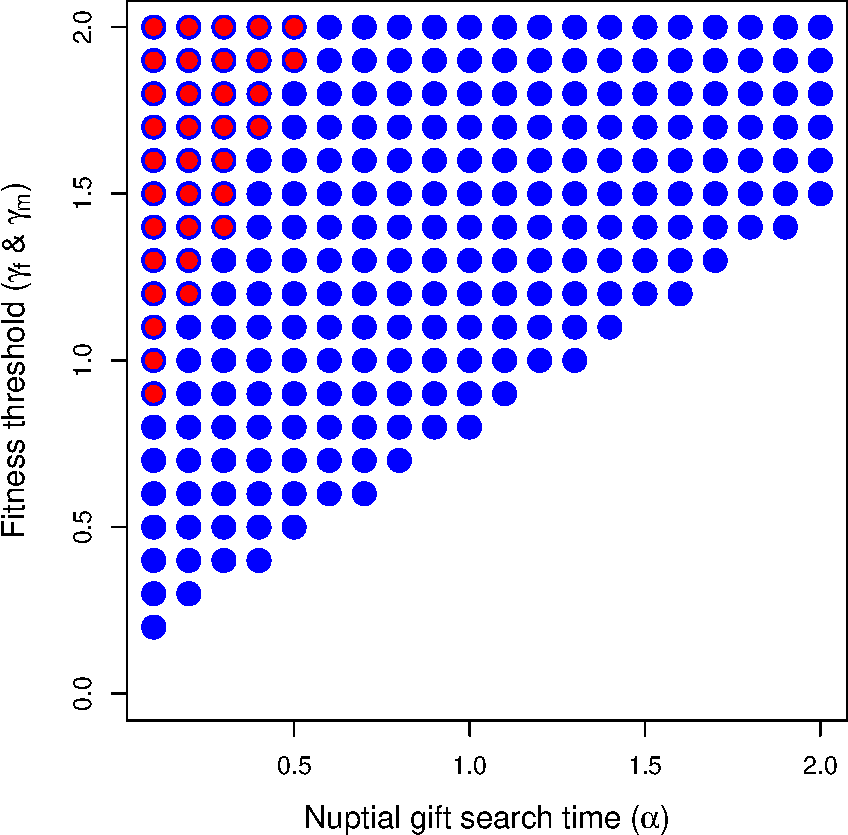
\includegraphics{SI_files/figure-latex/unnamed-chunk-5-1.pdf}
\caption{Figure S2.4 (\(\psi = 1\)): The coevolution of male search and
female choosiness as a function of nuptial gift search time
(\(\alpha\)). Points show where the lower 95\% confidence interval of
where male search (blue) exceeds zero, indicating evolution of
choosiness or nuptial gift search. Each point includes data from
approximately 100 replicate simulations with identical starting
conditions (some parameter combinations had fewer replicates, minimum
400). Red and blue lines show thresholds above which the mathematical
model predicts that females should be choosy and males should search,
respectively. Up to 1000 interactions occur between individuals in each
time step (\(\psi = 1\)), potentially resulting in a mating interaction.
The number of individuals in the population remained at or near carrying
capacity of \(K = 1000\). Expected female processing time was set to
\(T_{\mathrm{f}}=2\) time steps, and \(\gamma\) and \(\alpha\) values in
the range {[}0.0, 1.4{]} and {[}0.1, 1.2{]}, respectively, were used.}
\end{figure}

\captionsetup{labelformat=default}

\clearpage

\captionsetup{labelformat=empty}

\begin{figure}
\centering
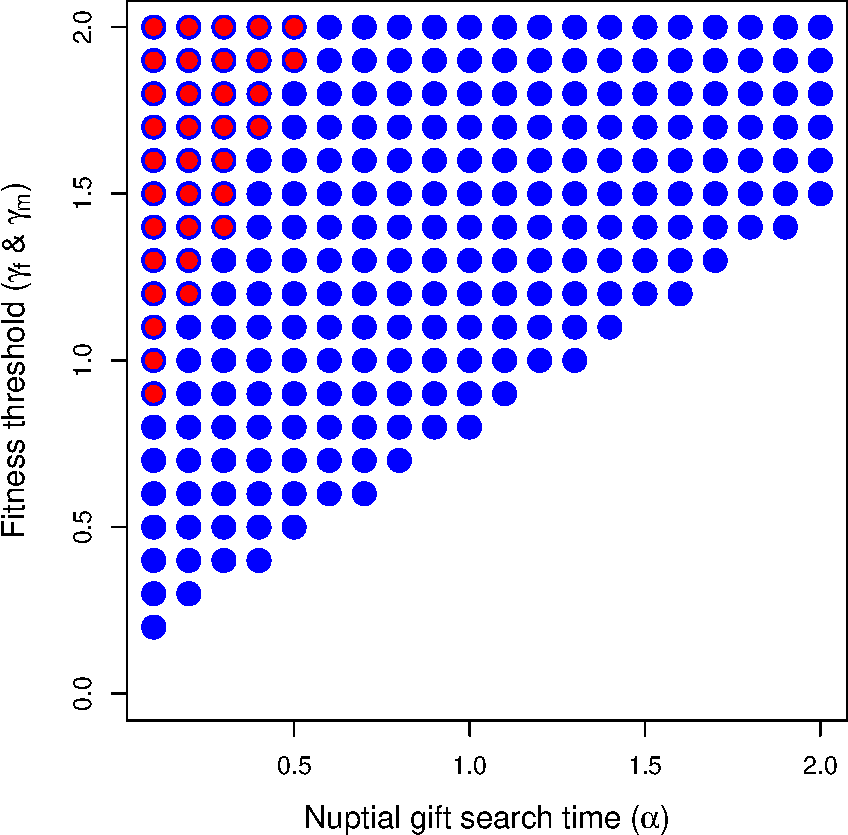
\includegraphics{SI_files/figure-latex/unnamed-chunk-6-1.pdf}
\caption{Figure S2.5 (\(\psi = 2\)): The coevolution of male search and
female choosiness as a function of nuptial gift search time
(\(\alpha\)). Points show where the lower 95\% confidence interval of
where male search (blue) exceeds zero, indicating evolution of
choosiness or nuptial gift search. Each point includes data from 100
replicate simulations with identical starting conditions (some parameter
combinations have fewer replicates). Red and blue lines show thresholds
above which the mathematical model predicts that females should be
choosy and males should search, respectively. Up to 2000 interactions
occur between individuals in each time step (\(\psi = 2\)), potentially
resulting in a mating interaction. The number of individuals in the
population remained at or near carrying capacity of \(K = 1000\).
Expected female processing time was set to \(T_{\mathrm{f}}=2\) time
steps, and \(\gamma\) and \(\alpha\) values in the range {[}0.0, 1.4{]}
and {[}0.1, 1.2{]}, respectively, were used.}
\end{figure}

\captionsetup{labelformat=default}

\clearpage

\captionsetup{labelformat=empty}

\begin{figure}
\centering
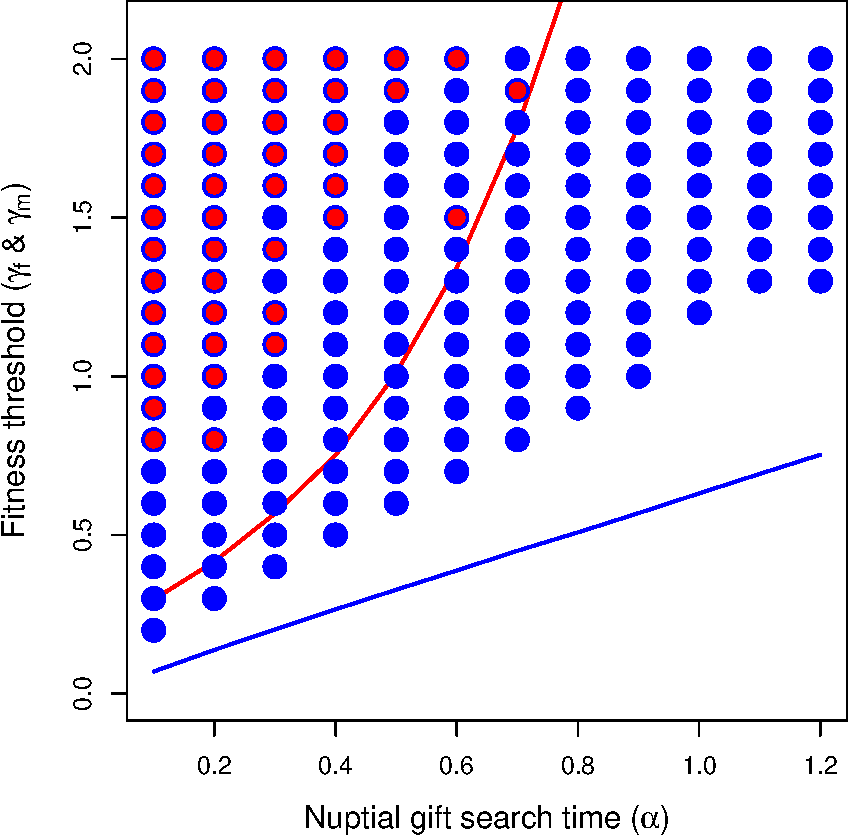
\includegraphics{SI_files/figure-latex/unnamed-chunk-7-1.pdf}
\caption{Figure S2.6 (\(\psi = 4\)): The coevolution of male search and
female choosiness as a function of nuptial gift search time
(\(\alpha\)). Points show where the lower 95\% confidence interval of
where male search (blue) exceeds zero, indicating evolution of
choosiness or nuptial gift search. Each point includes data from 100
replicate simulations with identical starting conditions (some parameter
combinations have fewer replicates). Red and blue lines show thresholds
above which the mathematical model predicts that females should be
choosy and males should search, respectively. Up to 4000 interactions
occur between individuals in each time step, potentially resulting in a
mating interaction (\(\psi = 4\)). The number of individuals in the
population remained at or near carrying capacity of \(K = 1000\).
Expected female processing time was set to \(T_{\mathrm{f}}=2\) time
steps, and \(\gamma\) and \(\alpha\) values in the range {[}0.0, 1.4{]}
and {[}0.1, 1.2{]}, respectively, were used.}
\end{figure}

\captionsetup{labelformat=default}

\clearpage

\captionsetup{labelformat=empty}

\begin{figure}
\centering
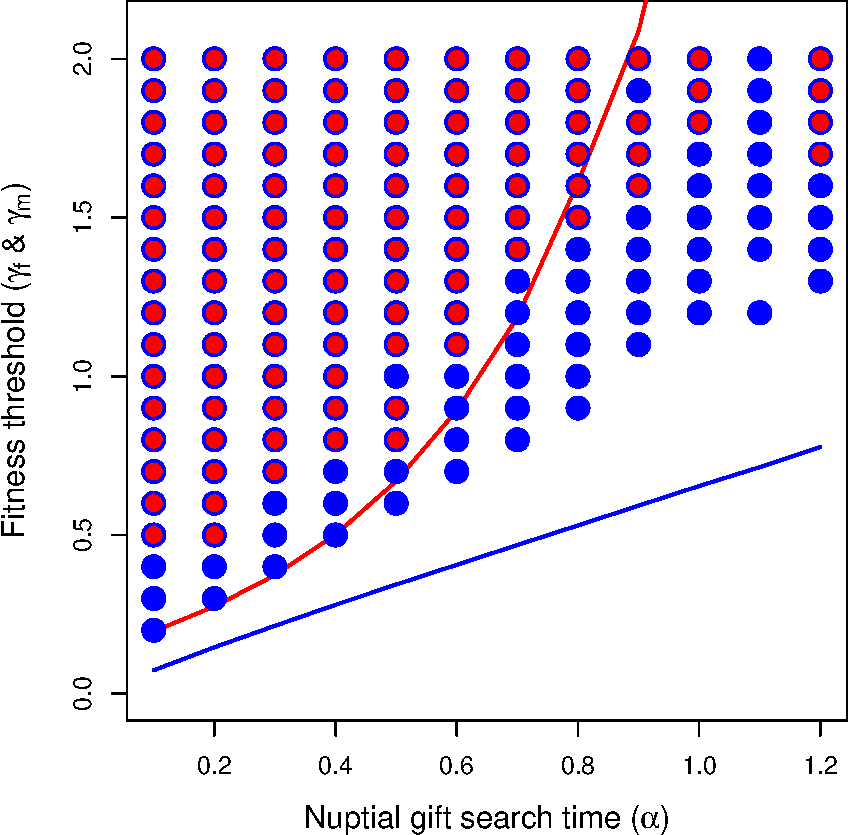
\includegraphics{SI_files/figure-latex/unnamed-chunk-8-1.pdf}
\caption{Figure S2.7 (\(\psi = 6\)): The coevolution of male search and
female choosiness as a function of nuptial gift search time
(\(\alpha\)). Points show where the lower 95\% confidence interval of
where male search (blue) exceeds zero, indicating evolution of
choosiness or nuptial gift search. Each point includes data from 100
replicate simulations with identical starting conditions (some parameter
combinations have fewer replicates). Red and blue lines show thresholds
above which the mathematical model predicts that females should be
choosy and males should search, respectively. Up to 6000 interactions
occur between individuals in each time step, potentially resulting in a
mating interaction (\(\psi = 6\)). The number of individuals in the
population remained at or near carrying capacity of \(K = 1000\).
Expected female processing time was set to \(T_{\mathrm{f}}=2\) time
steps, and \(\gamma\) and \(\alpha\) values in the range {[}0.0, 1.4{]}
and {[}0.1, 1.2{]}, respectively, were used.}
\end{figure}

\captionsetup{labelformat=default}

\clearpage

\captionsetup{labelformat=empty}

\begin{figure}
\centering
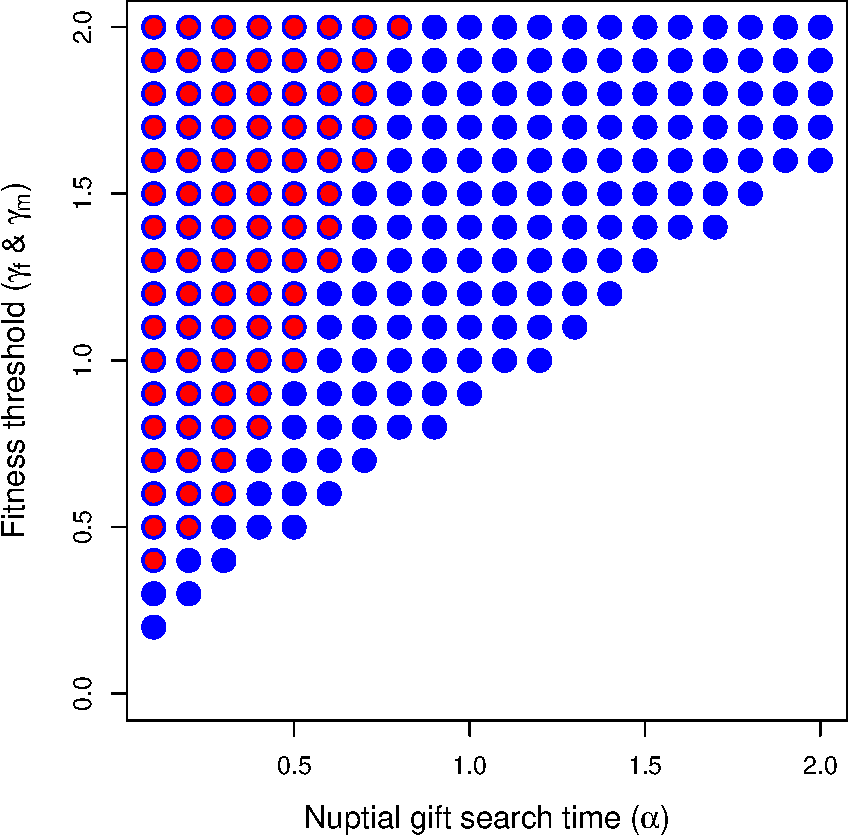
\includegraphics{SI_files/figure-latex/unnamed-chunk-9-1.pdf}
\caption{Figure S2.8 (\(T_{\mathrm{m}} = 0.5\)): The coevolution of male
search and female choosiness as a function of nuptial gift search time
(\(\alpha\)). Points show where the lower 95\% confidence interval of
where male search (blue) exceeds zero, indicating evolution of
choosiness or nuptial gift search. Each point includes data from 1600
replicate simulations with identical starting conditions. The red line
shows the threshold above which the mathematical model predicts that
females should be choosy (male thresholds for search are not shown
because simulations were initialised with males already searching for
nuptial gifts). Up to 3000 interactions occur between individuals in
each time step, potentially resulting in a mating interaction
(\(\psi = 3\)). The number of individuals in the population remained at
or near carrying capacity of \(K = 1000\). Expected female processing
time was set to \(T_{\mathrm{f}}=2\) time steps, and \(\gamma\) and
\(\alpha\) values in the range {[}0.0, 1.4{]} and {[}0.1, 1.2{]},
respectively, were used.}
\end{figure}

\captionsetup{labelformat=default}

\clearpage

\captionsetup{labelformat=empty}

\begin{figure}
\centering
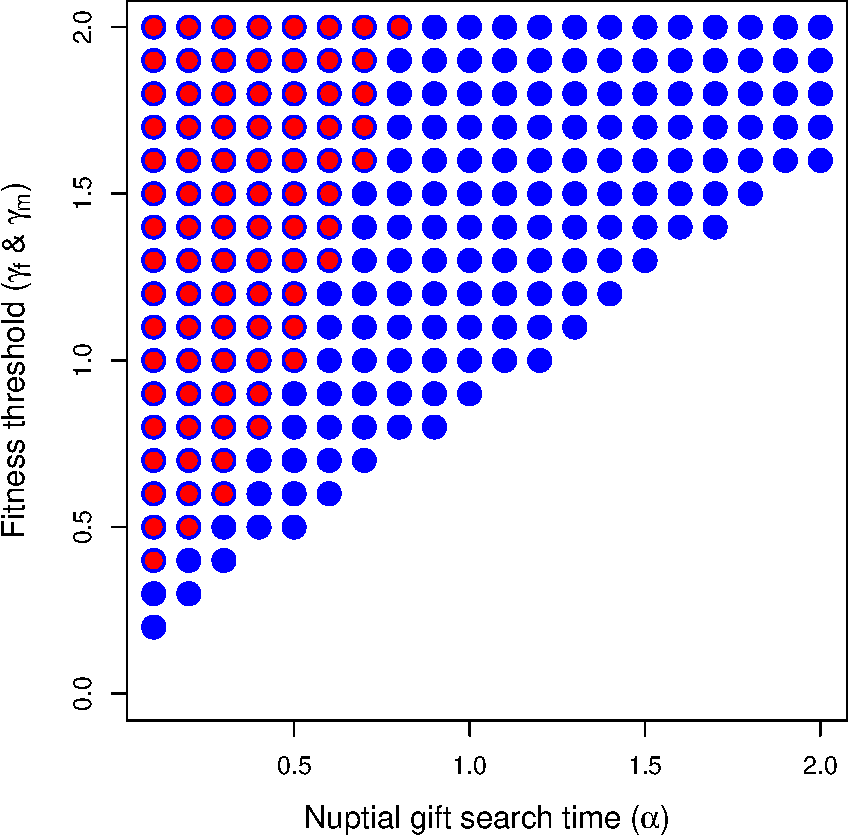
\includegraphics{SI_files/figure-latex/unnamed-chunk-10-1.pdf}
\caption{Figure S2.9 (\(T_{\mathrm{m}} = 2.5\)): The coevolution of male
search and female choosiness as a function of nuptial gift search time
(\(\alpha\)). Points show where the lower 95\% confidence interval of
where male search (blue) exceeds zero, indicating evolution of
choosiness or nuptial gift search. Each point includes data from 1600
replicate simulations with identical starting conditions. The red line
shows the threshold above which the mathematical model predicts that
females should be choosy (male thresholds for search are not shown
because simulations were initialised with males already searching for
nuptial gifts). Up to 3000 interactions occur between individuals in
each time step, potentially resulting in a mating interaction
(\(\psi = 3\)). The number of individuals in the population remained at
or near carrying capacity of \(K = 1000\). Expected female processing
time was set to \(T_{\mathrm{f}}=2\) time steps, and \(\gamma\) and
\(\alpha\) values in the range {[}0.0, 1.4{]} and {[}0.1, 1.2{]},
respectively, were used.}
\end{figure}

\captionsetup{labelformat=default}

\clearpage

\hypertarget{s3-alternative-derivation-of-male-fitness-threshold}{%
\subsection{S3: Alternative derivation of male fitness
threshold}\label{s3-alternative-derivation-of-male-fitness-threshold}}

In the main text, we assumed that males made the decision to search or
not search for a nuptial gift. The expected length of time for which
searching males are expected to remain outside of the mating pool is
\(E[T_{\mathrm{m}}] = \alpha\) (see Methods). Alternatively, we can
assume that males search for a period of \(T_{\mathrm{m}}\) and spend
this full duration of \(T_{\mathrm{m}}\) in the time-out phase, even if
they succeed in finding a nuptial gift. The probability that a male
obtains a nuptial gift during this time is modelled in Eq. 1,

\[P(G) = 1 - e^{-\frac{1}{\alpha}T_{\mathrm{m}}}.\]

In Eq. 1, \(\alpha\) is the amount of time expected to pass before a
male encounters a nuptial gift. We assume that a male will only enter
the mating pool with no gift if they are unsuccessful in obtaining a
gift, so the probability that a male obtains no gift after
\(T_{\mathrm{m}}\) is,

\[P(L) = e^{-\frac{1}{\alpha}T_{\mathrm{m}}}.\]

We assume that the fitness increments to offspring associated with
receiving a nuptial gift versus no nuptial gift are \(1 + \gamma\) and
1, respectively. The rate at which males increase their fitness can then
be defined as the expected fitness increment from their nuptial gift
search divided by \(T_{\mathrm{m}}\) plus the time spent in the mating
pool waiting to encounter a mate,

\[W_{\mathrm{m}} = \lambda \frac{P(G)\left(1 + \gamma\right) + P(L)}{T_{\mathrm{m}} + \left( \frac{\beta + 1}{R} \right)}.\]

Our objective now is to determine the conditions under which a focal
male increases its fitness by searching for a nuptial gift
(\(T_{\mathrm{m}}>0\)) in a population of resident males that do not
search (\(T_{\mathrm{m}}=0\)). Females are assumed to exhibit no choice
in males with versus without nuptial gifts. Under such conditions, male
fitness cannot be affected by female choice, so selection to increase
\(T_{\mathrm{m}}>0\) must be based solely on \(\alpha\), \(\beta\),
\(R\), and \(\gamma\).

To determine under what conditions male inclusive fitness increases with
nuptial gift search time, we can differentiate \(W_{\mathrm{m}}\) with
respect to \(T_{\mathrm{m}}\),

\[\frac{\partial W_{\mathrm{m}}}{\partial T_{\mathrm{m}}} = \lambda\frac{\gamma\left(\frac{\frac{T_{\mathrm{m}} + \frac{\beta + 1}{R}}{\alpha} + 1}{e^{\frac{1}{\alpha}T_{\mathrm{m}}}} - 1\right) - 1}{\left(T_{\mathrm{m}} + \frac{\beta + 1}{R} \right)^{2}}.\]

Because \(T_{\mathrm{m}} = 0\), the above simplifies,

\[\frac{\partial W_{\mathrm{m}}}{\partial T_{\mathrm{m}}} = \lambda \frac{\frac{R\gamma\left(\beta + 1\right)}{\alpha} - R^{2}}{\left(1 + \beta \right)^{2}}.\]

We can re-arrange the above,

\[\frac{\partial W_{\mathrm{m}}}{\partial T_{\mathrm{m}}} = \lambda \frac{R\gamma}{\alpha\left(\beta+1\right)} - \lambda\frac{R^{2}}{{\left(1 + \beta \right)^{2}}}.\]

Note that if \(R = 0\) or \(\lambda = 0\), then, trivially, no change in
fitness occurs (since females and males cannot mate or do not produce
offspring). Fitness is increased by searching for nuptial gifts when
\(\gamma\) is high, scaled by the expect search time needed to find a
nuptial gift. A second term on the right-hand side is subtracted, which
reflects a loss in fitness proportional to the encounter rate of
potential mates in the mating pool. The conditions under which male
inclusive fitness increases by searching for a nuptial gift are found by
setting \(\partial W_{\mathrm{m}}/\partial T_{\mathrm{m}} = 0\) and
solving for \(\gamma\) to get Eq. 2 in the main text.

\clearpage

\hypertarget{s4-operational-sex-ratio}{%
\subsection{S4: Operational sex ratio}\label{s4-operational-sex-ratio}}

We assume that the ratio of males to females is the same upon individual
maturation. Consequently, the operational sex ratio \(\beta\) will be a
function of \(R\), \(T_{\mathrm{f}}\), and \(T_{\mathrm{m}}\) because
these parameters determine the density of females and males in the
mating pool versus outside of the mating pool. We start with the
definition of \(\beta\) as being the probability of finding an
individual in time-in (\protect\hyperlink{ref-Kokko2001}{Kokko \&
Monaghan, 2001}),

\[\beta = \frac{\int_{t=0}^{\infty}P_{IM}(t)dt}{\int_{t=0}^{\infty}P_{IF}(t)dt}\]

We can substitute the equations for \(P_{IM}(t)\) and \(P_{IF}(t)\),
which define the probabilities of males and females being within the
mating pool at time \(t\), respectively.

We can therefore calculate \(\beta\) as below,

\[\beta = \frac{\left( \frac{\left(\frac{\beta + 1}{R}\right)}{T_{\mathrm{m}} + \left(\frac{\beta + 1}{R}\right)} \right)}{\left( \frac{\left(R \frac{\beta}{\beta + 1}\right)}{T_{\mathrm{f}} + \left(R \frac{\beta}{\beta + 1}\right)} \right)}.\]

This can be simplified,

\[\beta = \frac{\left(\beta\left(R + T_{f}\right) + T_{f}\right)\left(\beta + 1\right)}{\beta \left(R^{2}T_{m} + R\right) + \beta^{2}R}.\]

There is no closed form solution for \(\beta\), but a recursive
algorithm can be used to calculate \(\beta\) to an arbitrary degree of
precision.

\begin{Shaded}
\begin{Highlighting}[]
\NormalTok{recursive\_b }\OtherTok{\textless{}{-}} \ControlFlowTok{function}\NormalTok{(B, D, Tf, Tm, }\AttributeTok{crit =} \FloatTok{0.0001}\NormalTok{, }\AttributeTok{maxit =} \DecValTok{9999}\NormalTok{)\{}
\NormalTok{  conv }\OtherTok{\textless{}{-}} \DecValTok{1}\NormalTok{;}
\NormalTok{  iter }\OtherTok{\textless{}{-}} \DecValTok{0}\NormalTok{;}
  \ControlFlowTok{while}\NormalTok{(conv }\SpecialCharTok{\textgreater{}}\NormalTok{ crit }\SpecialCharTok{\&}\NormalTok{ iter }\SpecialCharTok{\textless{}}\NormalTok{ maxit)\{}
\NormalTok{    Fe   }\OtherTok{\textless{}{-}}\NormalTok{ D }\SpecialCharTok{*}\NormalTok{ (B }\SpecialCharTok{/}\NormalTok{ (}\DecValTok{1} \SpecialCharTok{+}\NormalTok{ B));}
\NormalTok{    Me   }\OtherTok{\textless{}{-}}\NormalTok{ (}\DecValTok{1} \SpecialCharTok{+}\NormalTok{ B) }\SpecialCharTok{/}\NormalTok{ D;}
\NormalTok{    Bn   }\OtherTok{\textless{}{-}}\NormalTok{ (Me }\SpecialCharTok{/}\NormalTok{ (Tm }\SpecialCharTok{+}\NormalTok{ Me)) }\SpecialCharTok{/}\NormalTok{ (Fe }\SpecialCharTok{/}\NormalTok{ (Tf }\SpecialCharTok{+}\NormalTok{ Fe));}
\NormalTok{    iter }\OtherTok{\textless{}{-}}\NormalTok{ iter }\SpecialCharTok{+} \DecValTok{1}\NormalTok{;}
\NormalTok{    conv }\OtherTok{\textless{}{-}} \FunctionTok{abs}\NormalTok{(Bn }\SpecialCharTok{{-}}\NormalTok{ B);}
\NormalTok{    B    }\OtherTok{\textless{}{-}}\NormalTok{ Bn;}
\NormalTok{  \}}
  \FunctionTok{return}\NormalTok{(}\FunctionTok{list}\NormalTok{(}\AttributeTok{B =}\NormalTok{ B, }\AttributeTok{conv =}\NormalTok{ conv, }\AttributeTok{iter =}\NormalTok{ iter));}
\NormalTok{\}}
\end{Highlighting}
\end{Shaded}

We used the above function to calculate values of \(\beta\) for the
analytical model.

\clearpage

\hypertarget{s5-estimation-of-key-model-parameters-using-experimental-data}{%
\subsection{S5: Estimation of key model parameters using experimental
data}\label{s5-estimation-of-key-model-parameters-using-experimental-data}}

Estimates showing the mean number of offspring produced by female
\emph{Pisaura mirabilis} that ate nuptial gifts and females who did not.
Means were calculated with raw data from Tuni \emph{et al.}
(\protect\hyperlink{ref-Tuni2013a}{2013}) and results are shown \(\pm\)
SE (Table 1). Under these assumptions, the relative gain in fitness from
receiving nuptial gifts for a female is,

\[\hat{\delta_\mathrm{f}} = \frac{25.74}{6.00} = 4.29\]

Since the baseline fitness is 1, the increase in fitness resulting from
a nuptial gift then becomes,

\[\hat{\gamma} = \hat{\delta_{\mathrm{f}}} - 1 = 3.29.\]

The value 3.29 was used to parameterise \(\gamma\) for a set of
simulations (Figure 4 in the main text).

\begin{longtable}[]{@{}
  >{\raggedright\arraybackslash}p{(\columnwidth - 4\tabcolsep) * \real{0.4024}}
  >{\raggedright\arraybackslash}p{(\columnwidth - 4\tabcolsep) * \real{0.2805}}
  >{\raggedright\arraybackslash}p{(\columnwidth - 4\tabcolsep) * \real{0.3171}}@{}}
\toprule
\begin{minipage}[b]{\linewidth}\raggedright
\end{minipage} & \begin{minipage}[b]{\linewidth}\raggedright
Received nuptial gift
\end{minipage} & \begin{minipage}[b]{\linewidth}\raggedright
Received no nuptial gift
\end{minipage} \\
\midrule
\endhead
Expected number of hatched eggs & \(25.74 \pm 0.96\) &
\(6.00 \pm 2.1\) \\
\bottomrule
\end{longtable}

Table 1: Estimates showing mean number of offspring produced by female
\emph{P. mirabilis} that ate nuptial gifts and females who did not.
Means were calculated with raw data from Tuni \emph{et al.}
(\protect\hyperlink{ref-Tuni2013a}{2013}) and results are shown \(\pm\)
SE.

\clearpage

\hypertarget{s6-separate-evolution-of-male-search-and-female-choice}{%
\subsection{S6: Separate evolution of male search and female
choice}\label{s6-separate-evolution-of-male-search-and-female-choice}}

We used the individual-based simulation model (see Supporting
Information S1) to unpack the effect of coevolution on the evolution of
male search and female choice. Here we replicated the simulations shown
in the main text under the condition where only one trait at a time was
allowed to evolve and studied how this affected the trait evolution.

First, we submitted a set of simulations wherein male search did not
evolve, but was fixed at different values (see Fig. S6.1). Next, we ran
the same set of simulations wherein male search evolved, but female
choice was not possible. The results thus show how each trait evolves in
the absence of any coevolution (Fig. S6.1).

\captionsetup{labelformat=empty}

\begin{figure}
\centering
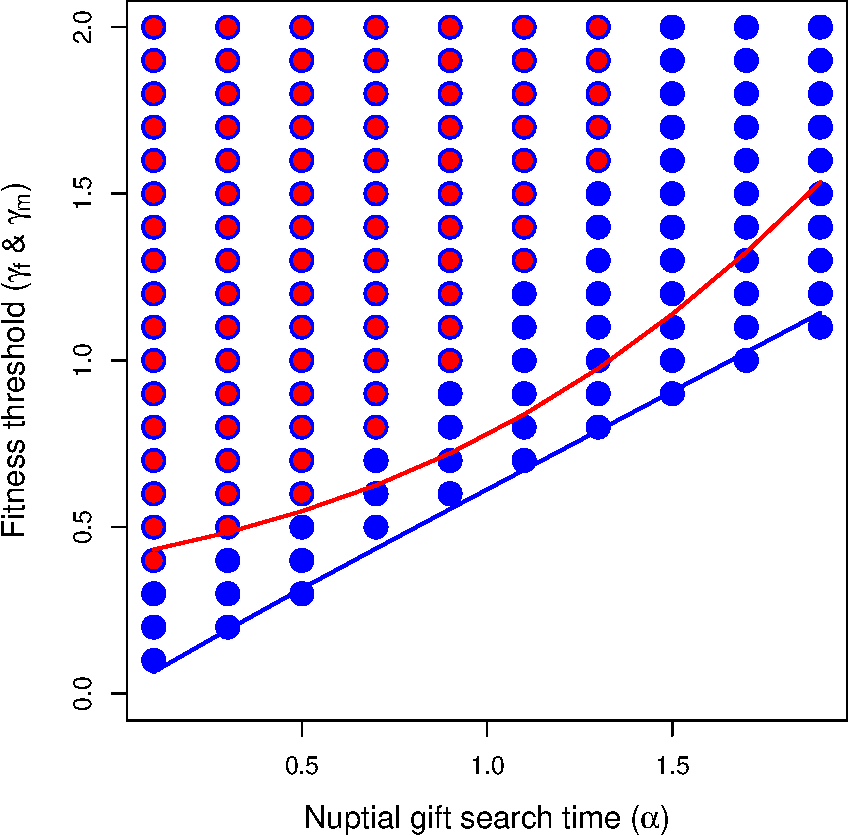
\includegraphics{SI_files/figure-latex/unnamed-chunk-12-1.pdf}
\caption{Figure S6.1: The separate evolution of male search and female
choosiness as a function of nuptial gift search time. Points show where
the lower 95\% confidence interval of male search (blue) and female
choosiness (red) exceeds zero, indicating evolution of nuptial gift
search or choosiness. Each point includes data from \(2 \times 1600\)
replicate simulations with identical starting conditions. In the first
batch, male search was constant and initialized at
\(T_{\mathrm{m}} = \alpha\), and female choice was evolving. In the
second batch, male search was evolving, and there was no option for
female choice. The parameters \(T_{\mathrm{f}}=2\), and \(\gamma\) and
\(\alpha\) values were set within the range {[}0.1, 2.0{]} and {[}0.3,
1.7{]}, respectively.}
\end{figure}

\captionsetup{labelformat=default}

\clearpage

\hypertarget{references}{%
\section*{References}\label{references}}
\addcontentsline{toc}{section}{References}

\hypertarget{refs}{}
\begin{CSLReferences}{0}{0}
\leavevmode\vadjust pre{\hypertarget{ref-Kokko2001}{}}%
Kokko, H. \& Monaghan, P. (2001)
\href{https://doi.org/10.1046/j.1461-0248.2001.00212.x}{{Predicting the
direction of sexual selection}}. \emph{Ecology Letters}, \textbf{4},
159--165.

\leavevmode\vadjust pre{\hypertarget{ref-Tuni2013a}{}}%
Tuni, C., Albo, M.J. \& Bilde, T. (2013)
\href{https://doi.org/10.1111/jeb.12137}{{Polyandrous females acquire
indirect benefits in a nuptial feeding species}}. \emph{Journal of
Evolutionary Biology}, \textbf{26}, 1307--1316.

\end{CSLReferences}

\end{document}
